\chapter{Noise Sources \& Noise Figure}
\label{ch:noise-figure}

\begin{nontechnical}

\textbf{Think of radio communication like having a conversation in a
crowded restaurant:}

\begin{itemize}
\tightlist
\item
  \textbf{Signal} = Your friend\textquotesingle s voice trying to reach
  you
\item
  \textbf{Noise} = All the background chatter, kitchen sounds, and air
  conditioning
\item
  \textbf{Noise Figure} = How much your hearing aids (or bad acoustics)
  make it harder to understand
\end{itemize}

\textbf{Why noise matters:} If the background noise is too loud, you
can\textquotesingle t hear your friend-\/-\/-even if
they\textquotesingle re shouting. Same with radio: if noise is too high,
the receiver can\textquotesingle t ``hear'' the signal, no matter how
powerful the transmitter.

\textbf{Key insights in plain English:}

\begin{enumerate}
\def\labelenumi{\arabic{enumi}.}
\item
  \textbf{Thermal noise is everywhere}: Just like atoms vibrating
  creates heat, electrons vibrating creates random electrical ``static''
  in every wire, antenna, and amplifier. This sets a fundamental
  limit-\/-\/-you can\textquotesingle t eliminate it, only work around
  it.
\item
  \textbf{The -174 dBm magic number}: This is the ``noise floor'' at
  room temperature for a 1 Hz bandwidth. Think of it as the quietest
  possible ``background hum'' in radio. Everything adds noise on top of
  this baseline.
\item
  \textbf{Amplifiers make noise worse}: Every amplifier adds its own
  noise (like a hearing aid with poor quality that adds hiss). The
  \textbf{noise figure} tells you how much worse the amplifier makes the
  signal-to-noise ratio.
\item
  \textbf{First stage is critical}: Just like you want your hearing aid
  right at your ear (not connected by a long cable), you want the first
  amplifier (Low-Noise Amplifier, or LNA) as close to the antenna as
  possible. Once noise is added early, you can\textquotesingle t remove
  it later.
\item
  \textbf{Wider bandwidth = more noise}: Like opening more windows lets
  in more outside noise, using a wider radio bandwidth lets in more
  thermal noise. This is why high-speed data links (wide bandwidth) need
  stronger signals than voice links (narrow bandwidth).
\end{enumerate}

\textbf{Real-world impact:} - \textbf{Satellite TV}: Premium receivers
have better (lower) noise figures, letting them work with smaller dishes
- \textbf{GPS}: Your phone\textquotesingle s GPS can detect signals
1,000\$\textbackslash times\$ weaker than WiFi because it fights noise
cleverly (spread spectrum) - \textbf{Deep space missions}: NASA uses
cryogenically-cooled amplifiers (like refrigerating your hearing aid!)
to reduce noise and hear probes billions of miles away

\textbf{Bottom line}: If you want to receive weak signals (long range,
small antenna, low power), you must minimize noise.
That\textquotesingle s why the first few inches of cable and the first
amplifier matter more than anything else in the receiver chain.
\end{nontechnical}

\section{Overview}

\textbf{Noise} is unwanted random signal that degrades communication
system performance.

\textbf{Key metrics}: - \textbf{Noise power} (N): Total noise at
receiver input (dBm, watts) - \textbf{Noise figure} (NF): How much a
component degrades SNR (dB) - \textbf{Noise temperature} (T\_e):
Equivalent thermal noise (Kelvin)

\textbf{Why it matters}:
\begin{itemize}
\item Determines \textbf{receiver sensitivity} (minimum detectable signal)
\item Sets \textbf{SNR} at demodulator input
\item Dominates link performance in low-signal scenarios (satellite, deep space)
\end{itemize}

\begin{keyconcept}
Lower noise = Better sensitivity = Longer range. The noise figure of the first amplifier (Low-Noise Amplifier, LNA) dominates the entire receiver chain performance due to the Friis formula.
\end{keyconcept}

\section{Mathematical Description}

\subsection{Thermal Noise}

\textbf{Fundamental noise source}: Random motion of charge carriers due
to thermal agitation

\subsubsection{Johnson-Nyquist Noise}

\textbf{Noise power} in resistor at temperature $T$:

\begin{equation}
N = k T B
\end{equation}
where:
\begin{itemize}
\item $N$ = noise power (watts)
\item $k = 1.38 \times 10^{-23}$ J/K (Boltzmann constant)
\item $T$ = absolute temperature (Kelvin)
\item $B$ = bandwidth (Hz)
\end{itemize}

\textbf{Standard reference temperature}: $T_0 = 290$ K (room temperature, $\approx 17°$C)

\subsubsection{Noise Power Spectral Density}

\textbf{Noise power per Hz}:

\begin{equation}
N_0 = k T
\end{equation}
where:
\begin{itemize}
\item $N_0$ = noise power spectral density (W/Hz)
\item $k$ = Boltzmann constant
\item $T$ = temperature (K)
\end{itemize}

\textbf{At reference temperature} $T_0 = 290$ K:

\begin{equation}
N_0 = 1.38 \times 10^{-23} \times 290 = 4 \times 10^{-21}~\text{W/Hz}
\end{equation}

\textbf{In dBm/Hz}:

\begin{equation}
N_0 = 10\log_{10}\left(\frac{4 \times 10^{-21}}{10^{-3}}\right) = -174~\text{dBm/Hz}
\end{equation}

\begin{calloutbox}{The Famous $-174$ dBm/Hz Thermal Noise Floor}
This is the fundamental noise floor at room temperature (290 K) in a 1 Hz bandwidth. All receiver noise calculations start from this baseline. It represents the minimum detectable signal level in an ideal noiseless receiver.
\end{calloutbox}

\subsubsection{Noise Power in Bandwidth B}

\begin{equation}
N = N_0 \times B = kTB
\end{equation}
where:
\begin{itemize}
\item $N$ = total noise power (watts)
\item $B$ = bandwidth (Hz)
\end{itemize}

\textbf{In logarithmic form (dBm)}:

\begin{equation}
N_{\text{dBm}} = -174 + 10\log_{10}(B)
\end{equation}

\textbf{Example}: 1 MHz bandwidth @ 290 K

\begin{equation}
N = -174 + 10\log_{10}(10^6) = -174 + 60 = -114~\text{dBm}
\end{equation}

\subsubsection{Typical Bandwidths and Noise
Power}\label{typical-bandwidths-and-noise-power}

{\def\LTcaptype{} % do not increment counter
\begin{longtable}[]{@{}lll@{}}
\toprule\noalign{}
System & Bandwidth & Noise Power @ 290 K \\
\midrule\noalign{}
\endhead
\bottomrule\noalign{}
\endlastfoot
\textbf{GPS C/A code} & 2 MHz & -111 dBm \\
\textbf{WiFi 20 MHz} & 20 MHz & -101 dBm \\
\textbf{LTE 10 MHz} & 10 MHz & -104 dBm \\
\textbf{DVB-S2 36 MHz} & 36 MHz & -98.4 dBm \\
\textbf{Radar (1 GHz pulse)} & 1 GHz & -84 dBm \\
\end{longtable}
}

\textbf{Key insight}: Wider bandwidth = More noise power

\subsection{Noise Figure (NF)}

\textbf{Definition}: Noise figure quantifies the \textbf{degradation of SNR} through a component or system.

\begin{equation}
F = \frac{\text{SNR}_{\text{in}}}{\text{SNR}_{\text{out}}}
\end{equation}
where:
\begin{itemize}
\item $F$ = noise factor (linear ratio)
\item $\text{SNR}_{\text{in}}$ = signal-to-noise ratio at input
\item $\text{SNR}_{\text{out}}$ = signal-to-noise ratio at output
\end{itemize}

\textbf{In logarithmic form (dB)}:

\begin{equation}
\text{NF}_{\text{dB}} = 10\log_{10}(F) = \text{SNR}_{\text{in,dB}} - \text{SNR}_{\text{out,dB}}
\end{equation}

\textbf{Physical Interpretation}:
\begin{itemize}
\item \textbf{NF = 0 dB} ($F = 1$): Ideal component (no noise added)
\item \textbf{NF = 3 dB} ($F = 2$): SNR halved (noise power doubled)
\item \textbf{NF = 10 dB} ($F = 10$): SNR reduced by $10\times$ (noise power increased $10\times$)
\end{itemize}

\subsubsection{Noise Figure vs Noise Factor}

\textbf{Noise factor} ($F$): Linear ratio

\textbf{Noise figure} (NF): Logarithmic (dB)

\begin{equation}
\text{NF}_{\text{dB}} = 10\log_{10}(F)
\end{equation}

\textbf{Example}: $F = 2$ $\rightarrow$ $\text{NF} = 3$ dB

\subsubsection{Typical Noise Figures}\label{typical-noise-figures}

{\def\LTcaptype{} % do not increment counter
\begin{longtable}[]{@{}lll@{}}
\toprule\noalign{}
Component & Noise Figure (dB) & Notes \\
\midrule\noalign{}
\endhead
\bottomrule\noalign{}
\endlastfoot
\textbf{Passive cable} & Loss in dB & Lossy line: NF = loss \\
\textbf{Ideal amplifier} & 0 & Theoretical only \\
\textbf{Cryogenic LNA} & 0.3-0.8 & Cooled to 20-80 K \\
\textbf{Premium LNA} & 0.8-1.5 & GaAs HEMT, room temp \\
\textbf{Good LNA} & 1.5-3 & Typical satellite ground \\
\textbf{WiFi/cellular front-end} & 5-9 & Consumer devices \\
\textbf{Mixer (passive)} & 6-10 & Diode mixer \\
\textbf{Mixer (active)} & 10-15 & Gilbert cell \\
\end{longtable}
}

\subsection{Noise Temperature}

\textbf{Alternative representation}: Equivalent input noise temperature

\begin{equation}
T_e = T_0 (F - 1)
\end{equation}
where:
\begin{itemize}
\item $T_e$ = equivalent noise temperature (K)
\item $T_0 = 290$ K (reference temperature)
\item $F$ = noise factor
\end{itemize}

\textbf{Inverse relationship}:

\begin{equation}
F = 1 + \frac{T_e}{T_0}
\end{equation}

\begin{equation}
\text{NF}_{\text{dB}} = 10\log_{10}\left(1 + \frac{T_e}{290}\right)
\end{equation}

\subsubsection{Noise Figure \$\textbackslash leftrightarrow\$ Noise
Temperature}\label{noise-figure-noise-temperature}

{\def\LTcaptype{} % do not increment counter
\begin{longtable}[]{@{}lll@{}}
\toprule\noalign{}
NF (dB) & Noise Factor F & \(T_e\) (K) \\
\midrule\noalign{}
\endhead
\bottomrule\noalign{}
\endlastfoot
0 & 1 & 0 \\
0.5 & 1.12 & 35 \\
1 & 1.26 & 75 \\
2 & 1.58 & 169 \\
3 & 2 & 290 \\
6 & 4 & 870 \\
10 & 10 & 2610 \\
\end{longtable}
}

\textbf{Usage}: Satellite and radio astronomy communities prefer $T_e$, RF engineers prefer NF.

\section{Cascaded Systems and Friis Formula}

\subsection{Friis Formula for Cascaded Stages}

For a multi-stage system with amplifiers, mixers, and filters in series:

\begin{equation}
F_{\text{total}} = F_1 + \frac{F_2 - 1}{G_1} + \frac{F_3 - 1}{G_1 G_2} + \frac{F_4 - 1}{G_1 G_2 G_3} + \cdots
\end{equation}
where:
\begin{itemize}
\item $F_{\text{total}}$ = total system noise factor
\item $F_i$ = noise factor of stage $i$ (linear ratio)
\item $G_i$ = power gain of stage $i$ (linear ratio, not dB)
\end{itemize}

\textbf{In logarithmic form}:

\begin{equation}
\text{NF}_{\text{total,dB}} = 10\log_{10}(F_{\text{total}})
\end{equation}

\subsection{Key Insights from Friis Formula}

\begin{warningbox}
\textbf{Three Critical Design Rules:}

\begin{enumerate}
\item \textbf{First stage dominates}: $F_1$ appears without division $\rightarrow$ \textbf{LNA is critical!}
\item \textbf{High gain helps}: Later stages are divided by $G_1 G_2 \cdots$ $\rightarrow$ Less impact on total NF
\item \textbf{Avoid loss before LNA}: Cable loss before the LNA directly degrades system NF by the same amount
\end{enumerate}
\end{warningbox}

\subsection{Worked Example 1: Cable Before LNA (Poor Design)}

\textbf{Configuration}:
\begin{enumerate}
\item \textbf{Cable}: Loss = 2 dB ($F = 1.58$, $G = 0.63$)
\item \textbf{LNA}: NF = 1 dB ($F = 1.26$), Gain = 20 dB ($G = 100$)
\item \textbf{Mixer}: NF = 10 dB ($F = 10$), Gain = $-6$ dB ($G = 0.25$)
\end{enumerate}

\textbf{Solution}:

Using Friis formula:
\begin{equation}
F_{\text{total}} = 1.58 + \frac{1.26 - 1}{0.63} + \frac{10 - 1}{0.63 \times 100}
\end{equation}

\begin{equation}
F_{\text{total}} = 1.58 + 0.41 + 0.14 = 2.13
\end{equation}

\begin{equation}
\text{NF}_{\text{total}} = 10\log_{10}(2.13) = 3.3~\text{dB}
\end{equation}

\textbf{Analysis}: System noise figure is dominated by the 2 dB cable loss before the LNA!

\subsection{Worked Example 2: LNA Before Cable (Best Practice)}

\textbf{Configuration}:
\begin{enumerate}
\item \textbf{LNA}: NF = 1 dB ($F = 1.26$), Gain = 20 dB ($G = 100$)
\item \textbf{Cable}: Loss = 2 dB ($F = 1.58$, $G = 0.63$)
\item \textbf{Mixer}: NF = 10 dB ($F = 10$), Gain = $-6$ dB ($G = 0.25$)
\end{enumerate}

\textbf{Solution}:

Using Friis formula:
\begin{equation}
F_{\text{total}} = 1.26 + \frac{1.58 - 1}{100} + \frac{10 - 1}{100 \times 0.63}
\end{equation}

\begin{equation}
F_{\text{total}} = 1.26 + 0.0058 + 0.14 = 1.41
\end{equation}

\begin{equation}
\text{NF}_{\text{total}} = 10\log_{10}(1.41) = 1.5~\text{dB}
\end{equation}

\begin{calloutbox}{Design Lesson}
\textbf{1.8 dB improvement!} Placing the LNA at the antenna (before the cable) dramatically improves system noise figure. The LNA's high gain ($G = 100$) reduces the impact of the cable loss from 2.0 dB to only 0.006 dB in the total NF calculation.
\end{calloutbox}

\subsection{Worked Example 3: Two-Stage LNA}

\textbf{Configuration}:
\begin{enumerate}
\item \textbf{LNA1}: NF = 0.8 dB ($F = 1.2$), Gain = 15 dB ($G = 31.6$)
\item \textbf{LNA2}: NF = 1.5 dB ($F = 1.41$), Gain = 20 dB ($G = 100$)
\item \textbf{Mixer}: NF = 10 dB ($F = 10$), Gain = $-6$ dB ($G = 0.25$)
\end{enumerate}

\textbf{Solution}:

Using Friis formula:
\begin{equation}
F_{\text{total}} = 1.2 + \frac{1.41 - 1}{31.6} + \frac{10 - 1}{31.6 \times 100}
\end{equation}

\begin{equation}
F_{\text{total}} = 1.2 + 0.013 + 0.0028 = 1.216
\end{equation}

\begin{equation}
\text{NF}_{\text{total}} = 10\log_{10}(1.216) = 0.85~\text{dB}
\end{equation}

\textbf{Analysis}: Excellent performance! The high-gain first-stage LNA effectively isolates the system from later stage noise contributions.

\subsection{Performance Comparison}

The following diagram compares the total noise figure for the three receiver configurations:

\begin{center}
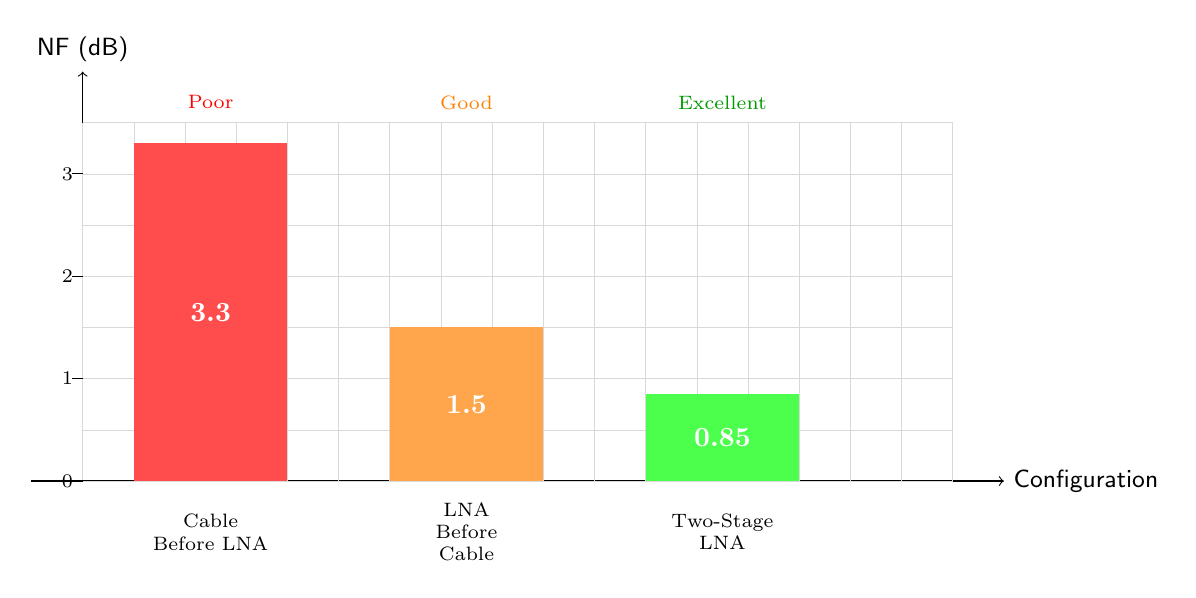
\begin{tikzpicture}[scale=1.3]
% Axes
\draw[->] (0,0) -- (0,4) node[above] {\sffamily\small NF (dB)};
\draw[->] (-0.5,0) -- (9,0) node[right] {\sffamily\small Configuration};

% Grid
\draw[very thin,gray!30] (0,0) grid[step=0.5] (8.5,3.5);

% Bars
\fill[red!70] (0.5,0) rectangle (2,3.3) node[midway, white, font=\bfseries] {3.3};
\fill[orange!70] (3,0) rectangle (4.5,1.5) node[midway, white, font=\bfseries] {1.5};
\fill[green!70] (5.5,0) rectangle (7,0.85) node[midway, white, font=\bfseries] {0.85};

% Labels
\node[font=\scriptsize, align=center, text width=1.5cm] at (1.25,-0.5) {Cable\\Before LNA};
\node[font=\scriptsize, align=center, text width=1.5cm] at (3.75,-0.5) {LNA\\Before Cable};
\node[font=\scriptsize, align=center, text width=1.5cm] at (6.25,-0.5) {Two-Stage\\LNA};

% Y-axis labels
\foreach \y in {0,1,2,3}
    \draw (-0.1,\y) -- (0,\y) node[left, font=\scriptsize] {\y};

% Annotations
\node[font=\scriptsize, text=red] at (1.25,3.7) {Poor};
\node[font=\scriptsize, text=orange] at (3.75,3.7) {Good};
\node[font=\scriptsize, text=green!60!black] at (6.25,3.7) {Excellent};
\end{tikzpicture}
\end{center}

\subsection{Cascaded System Architecture}

The following diagram illustrates a typical receiver chain showing how noise accumulates through cascaded stages:

\begin{center}
\begin{tikzpicture}[
  block/.style={rectangle, draw, minimum width=2.2cm, minimum height=1cm, font=\sffamily\small},
  node distance=2.2cm,
  font=\small
]
\node (input) {\sffamily Antenna\\Input};
\node[block, right of=input, node distance=2.8cm] (lna) {LNA\\$F_1, G_1$};
\node[block, right of=lna, node distance=3cm] (cable) {Cable\\$F_2, G_2$};
\node[block, right of=cable, node distance=3cm] (mixer) {Mixer\\$F_3, G_3$};
\node[block, right of=mixer, node distance=3cm] (if) {IF Amp\\$F_4, G_4$};
\node[right of=if, node distance=2.8cm] (output) {\sffamily Baseband\\Output};

% Signal flow arrows
\draw[->,thick] (input) -- (lna);
\draw[->,thick] (lna) -- (cable);
\draw[->,thick] (cable) -- (mixer);
\draw[->,thick] (mixer) -- (if);
\draw[->,thick] (if) -- (output);

% Noise contributions
\node[below=0.3cm of lna, font=\scriptsize, text=red] {$F_1$ (dominant)};
\node[below=0.3cm of cable, font=\scriptsize, text=orange] {$\frac{F_2-1}{G_1}$};
\node[below=0.3cm of mixer, font=\scriptsize, text=blue] {$\frac{F_3-1}{G_1G_2}$};
\node[below=0.3cm of if, font=\scriptsize, text=gray] {$\frac{F_4-1}{G_1G_2G_3}$};

% Friis formula annotation
\node[below=1.5cm of cable, font=\scriptsize, align=center, text width=6cm] {
Friis Formula: $F_{\text{tot}} = F_1 + \frac{F_2-1}{G_1} + \frac{F_3-1}{G_1G_2} + \cdots$
};
\end{tikzpicture}
\end{center}

\section{System Noise Temperature}

\textbf{Total noise temperature} of cascaded system:

\begin{equation}
T_{\text{sys}} = T_{\text{ant}} + T_e
\end{equation}
where:
\begin{itemize}
\item $T_{\text{sys}}$ = total system noise temperature (K)
\item $T_{\text{ant}}$ = antenna noise temperature (K)
\item $T_e$ = receiver equivalent noise temperature (K)
\end{itemize}

\subsubsection{Antenna Noise
Temperature}\label{antenna-noise-temperature}

\textbf{Antenna picks up thermal radiation} from environment:

\textbf{Sources}: - \textbf{Sky}: 3-300 K (depends on frequency,
elevation) - \textbf{Ground}: 290 K (room temperature) - \textbf{Sun}:
\textasciitilde10,000 K (if pointed directly) - \textbf{Cosmic
background}: 2.7 K (everywhere)

\textbf{Typical values}:

{\def\LTcaptype{} % do not increment counter
\begin{longtable}[]{@{}llll@{}}
\toprule\noalign{}
Scenario & Frequency & Elevation & \(T_{\text{ant}}\) (K) \\
\midrule\noalign{}
\endhead
\bottomrule\noalign{}
\endlastfoot
\textbf{Deep space} & Any & - & 3-5 \\
\textbf{Satellite (clear sky)} & 1-10 GHz &
30\$\^{}\textbackslash circ\$ & 20-50 \\
\textbf{Satellite (rain)} & 12 GHz & 30\$\^{}\textbackslash circ\$ &
100-200 \\
\textbf{Terrestrial} & Any & Horizon & 290 \\
\end{longtable}
}

\subsection{G/T Ratio (Figure of Merit)}

\textbf{System performance metric} for satellite ground stations:

\begin{equation}
\frac{G}{T} = G_r - 10\log_{10}(T_{\text{sys}})
\end{equation}
where:
\begin{itemize}
\item $G/T$ = system figure of merit (dB/K)
\item $G_r$ = receive antenna gain (dBi)
\item $T_{\text{sys}}$ = system noise temperature (K)
\end{itemize}

\textbf{Interpretation}: Higher $G/T$ = Better sensitivity

\textbf{Example}: 3 m Ku-band dish with LNA at feed
\begin{itemize}
\item Antenna gain: 48 dBi
\item Antenna temp: 30 K (clear sky, $30°$ elevation)
\item LNA NF: 0.8 dB $\rightarrow$ $T_e = 55$ K
\item $T_{\text{sys}} = 30 + 55 = 85$ K
\end{itemize}

\begin{equation}
\frac{G}{T} = 48 - 10\log_{10}(85) = 48 - 19.3 = 28.7~\text{dB/K}
\end{equation}

\textbf{Typical G/T values}:
\begin{itemize}
\item \textbf{VSAT terminals} (0.6-1.2 m): 10-20 dB/K
\item \textbf{Professional earth stations} (3-9 m): 25-35 dB/K
\item \textbf{Large observatories} (25+ m): 40-60 dB/K
\end{itemize}

\section{Other Noise Sources}

\subsection{Noise Source Categories}

The following diagram illustrates different noise sources and their frequency dependencies:

\begin{center}
\begin{tikzpicture}[scale=1.2]
% Axes
\draw[->] (0,0) -- (10,0) node[right] {\sffamily\small Frequency};
\draw[->] (0,0) -- (0,5) node[above] {\sffamily\small Noise Power};

% Flicker noise (1/f)
\draw[thick, red, domain=0.5:3] plot (\x, {3/\x + 1.5});
\node[red, font=\scriptsize] at (1.5,3.5) {Flicker $(1/f)$};

% Thermal noise (flat)
\draw[thick, blue] (0.5,1.5) -- (9.5,1.5);
\node[blue, font=\scriptsize] at (7,2) {Thermal (white)};

% Shot noise (flat)
\draw[thick, green!60!black, dashed] (0.5,2.2) -- (9.5,2.2);
\node[green!60!black, font=\scriptsize] at (7,2.7) {Shot (white)};

% Phase noise (near carrier)
\draw[thick, orange, domain=4:6] plot (\x, {0.8/(\x-4.5)^2 + 1.5});
\node[orange, font=\scriptsize] at (5,3.8) {Phase};
\draw[dashed, gray] (5,0) -- (5,1.5) node[below, font=\scriptsize] {$f_c$};

% Frequency bands
\node[font=\scriptsize] at (1.5,-0.5) {Audio};
\node[font=\scriptsize] at (5,-0.5) {RF/IF};
\node[font=\scriptsize] at (8.5,-0.5) {Broadband};

% Grid
\draw[very thin,gray!30] (0,0) grid[step=0.5] (10,5);
\end{tikzpicture}
\end{center}

\subsection{Shot Noise}

\textbf{Due to discrete nature of charge carriers}:

\begin{equation}
i_n^2 = 2 q I_{\text{DC}} B
\end{equation}
where:
\begin{itemize}
\item $i_n$ = RMS noise current (A)
\item $q = 1.6 \times 10^{-19}$ C (electron charge)
\item $I_{\text{DC}}$ = DC current (A)
\item $B$ = bandwidth (Hz)
\end{itemize}

\textbf{Significant in}: Photodetectors, diodes, low-current circuits

\textbf{Example}: Photodiode with 1 mA DC current, 1 MHz BW

\begin{equation}
i_n = \sqrt{2 \times 1.6 \times 10^{-19} \times 10^{-3} \times 10^6} = 5.7 \times 10^{-10}~\text{A}_{\text{rms}}
\end{equation}

\subsection{Flicker Noise (1/f Noise)}

\textbf{Low-frequency noise}, power inversely proportional to frequency:

\begin{equation}
S(f) \propto \frac{1}{f}
\end{equation}
where:
\begin{itemize}
\item $S(f)$ = noise power spectral density
\item $f$ = frequency (Hz)
\end{itemize}

\textbf{Significant below}: $< 1$ kHz (audio, low-IF systems)

\textbf{Mitigation}: Use higher IF, differential circuits, chopper stabilization

\subsection{Phase Noise}

\textbf{Oscillator noise} causes frequency jitter, specified as $\mathcal{L}(f_m)$ (dBc/Hz at offset $f_m$ from carrier).

\textbf{Example}: Satellite LO @ 10 GHz
\begin{itemize}
\item Phase noise: $-90$ dBc/Hz @ 10 kHz offset
\item Degrades SNR in adjacent channels
\item Critical for coherent demodulation
\end{itemize}

\subsection{Quantization Noise}

\textbf{Analog-to-digital conversion} introduces rounding error:

\begin{equation}
\text{SNR}_{\text{quant}} = 6.02n + 1.76
\end{equation}
where:
\begin{itemize}
\item $\text{SNR}_{\text{quant}}$ = quantization SNR (dB)
\item $n$ = number of ADC bits
\end{itemize}

\textbf{Example}: 12-bit ADC

\begin{equation}
\text{SNR}_{\text{quant}} = 6.02 \times 12 + 1.76 = 74~\text{dB}
\end{equation}

\textbf{Implication}: Need enough ADC bits to avoid degrading RF SNR.

\subsection{Intermodulation Distortion (IMD)}

\textbf{Non-linear components} create spurious products.

\textbf{Two-tone test}: Inputs at $f_1$ and $f_2$ produce third-order products at $2f_1 - f_2$ and $2f_2 - f_1$.

\textbf{IP3} (Third-order intercept point):

\begin{equation}
\text{IMD3}_{\text{dBc}} = 2(P_{\text{IP3}} - P_{\text{in}})
\end{equation}
where:
\begin{itemize}
\item $\text{IMD3}_{\text{dBc}}$ = third-order IMD level relative to carrier (dBc)
\item $P_{\text{IP3}}$ = third-order intercept point (dBm)
\item $P_{\text{in}}$ = input power (dBm)
\end{itemize}

\textbf{Example}: Mixer with IP3 = $+10$ dBm, input = $-20$ dBm

\begin{equation}
\text{IMD3} = 2(10 - (-20)) = 60~\text{dBc}
\end{equation}

\textbf{Implication}: Strong interferers create in-band noise.

\subsection{Atmospheric Noise}

\textbf{Natural sources}:
\begin{itemize}
\item \textbf{Lightning}: Dominates $< 30$ MHz (HF, VHF)
\item \textbf{Cosmic noise}: Galactic background (0.1-3 GHz)
\item \textbf{Solar noise}: Sun radiation (all frequencies)
\end{itemize}

\textbf{External noise temperature} $T_{\text{ext}}$:

{\def\LTcaptype{} % do not increment counter
\begin{longtable}[]{@{}lll@{}}
\toprule\noalign{}
Frequency & \(T_{\text{ext}}\) (K) & Dominant Source \\
\midrule\noalign{}
\endhead
\bottomrule\noalign{}
\endlastfoot
10 MHz & 10,000-100,000 & Lightning (HF) \\
100 MHz & 1,000-10,000 & Galactic noise \\
1 GHz & 10-100 & Cosmic background \\
10 GHz & 3-30 & Sky temp (clear) \\
60 GHz & 100-300 & Atmospheric O\textbackslash textsubscript\{2\} \\
\end{longtable}
}

\textbf{Antenna noise temperature}:

\begin{equation}
T_{\text{ant}} = T_{\text{ext}} \eta + T_0 (1 - \eta)
\end{equation}
where:
\begin{itemize}
\item $T_{\text{ant}}$ = antenna noise temperature (K)
\item $T_{\text{ext}}$ = external noise temperature (K)
\item $\eta$ = antenna efficiency (0 to 1)
\item $T_0 = 290$ K (reference temperature)
\end{itemize}

\subsection{Man-Made Noise}

\textbf{Interference from}: Power lines, electric motors, computers, switching power supplies

\textbf{Impulsive noise}: Short bursts (microseconds) with high peak power

\textbf{Mitigation}: Filtering, shielding, time diversity (retransmission)

\section{Receiver Sensitivity and Performance}

\subsection{Receiver Sensitivity Calculation}

\textbf{Minimum detectable signal} for target SNR:

\begin{equation}
P_{\text{min}} = N + \text{NF} + \text{SNR}_{\text{req}} + L_{\text{impl}}
\end{equation}
where (all in dB):
\begin{itemize}
\item $P_{\text{min}}$ = minimum detectable signal (dBm)
\item $N = -174 + 10\log_{10}(B)$ = thermal noise in bandwidth $B$ (dBm)
\item $\text{NF}$ = receiver noise figure (dB)
\item $\text{SNR}_{\text{req}}$ = required SNR for demodulation (dB)
\item $L_{\text{impl}}$ = implementation loss (1-3 dB typical)
\end{itemize}

\subsection{Worked Example: GPS Receiver}

\textbf{Given Parameters}:
\begin{itemize}
\item Bandwidth: 2 MHz (C/A code)
\item NF: 3 dB (typical GPS front-end)
\item $\text{SNR}_{\text{req}}$: $-20$ dB (spread spectrum processing gain 43 dB)
\item Implementation loss: 2 dB
\item C/N$_0$ requirement: 33 dB-Hz (acquisition), 28 dB-Hz (tracking)
\end{itemize}

\textbf{Step 1: Calculate thermal noise}:

\begin{equation}
N = -174 + 10\log_{10}(2 \times 10^6) = -174 + 63 = -111~\text{dBm}
\end{equation}

\textbf{Step 2: Calculate sensitivity (method 1)}:

\begin{equation}
P_{\text{min}} = N + \text{NF} + \text{SNR}_{\text{req}} + L_{\text{impl}}
\end{equation}

\begin{equation}
P_{\text{min}} = -111 + 3 + (-20) + 2 = -126~\text{dBm}
\end{equation}

\textbf{Step 3: Alternate method using C/N$_0$ metric}:

\begin{equation}
P_{\text{min}} = -174 + \text{C/N}_0 + \text{NF} + L_{\text{impl}}
\end{equation}

\begin{equation}
P_{\text{min}} = -174 + 33 + 3 + 2 = -136~\text{dBm}
\end{equation}

\begin{calloutbox}{GPS Link Margin}
\textbf{Typical GPS signal}: $-130$ dBm (open sky) $\rightarrow$ 6 dB margin for acquisition. This margin allows GPS to work indoors near windows and in light foliage.
\end{calloutbox}

\subsection{Worked Example: Satellite DVB-S2 Receiver}

\textbf{Given Parameters}:
\begin{itemize}
\item Bandwidth: 36 MHz
\item NF: 1.5 dB (LNA at feed)
\item Modulation: QPSK 3/4 with LDPC coding
\item $\text{SNR}_{\text{req}}$: 6.5 dB (for BER $< 10^{-7}$ post-FEC)
\item Implementation loss: 1.5 dB
\end{itemize}

\textbf{Step 1: Calculate thermal noise}:

\begin{equation}
N = -174 + 10\log_{10}(36 \times 10^6) = -174 + 75.6 = -98.4~\text{dBm}
\end{equation}

\textbf{Step 2: Calculate sensitivity}:

\begin{equation}
P_{\text{min}} = N + \text{NF} + \text{SNR}_{\text{req}} + L_{\text{impl}}
\end{equation}

\begin{equation}
P_{\text{min}} = -98.4 + 1.5 + 6.5 + 1.5 = -88.9~\text{dBm}
\end{equation}

\textbf{Result}: Link budget must deliver $> -88.9$ dBm at LNB output for proper operation.

\section{Noise Figure Measurement}

\subsection{Y-Factor Method}

\textbf{Standard technique} using hot/cold loads:

\textbf{Procedure}:
\begin{enumerate}
\item Measure noise power with \textbf{hot load} ($T_h = 290$ K): $P_h$
\item Measure noise power with \textbf{cold load} ($T_c = 77$ K, liquid N$_2$): $P_c$
\item Calculate \textbf{Y-factor}:
\end{enumerate}

\begin{equation}
Y = \frac{P_h}{P_c}
\end{equation}

\begin{enumerate}
\setcounter{enumi}{3}
\item Calculate \textbf{noise figure}:
\end{enumerate}

\begin{equation}
\text{NF} = 10\log_{10}\left(\frac{T_h - YT_c}{290(Y-1)}\right)
\end{equation}

\textbf{Example}: $P_h = 100$ units, $P_c = 80$ units

\begin{equation}
Y = \frac{100}{80} = 1.25
\end{equation}

\begin{equation}
\text{NF} = 10\log_{10}\left(\frac{290 - 1.25 \times 77}{290 \times 0.25}\right) = 1.8~\text{dB}
\end{equation}

\subsection{Noise Source Method}

\textbf{Use calibrated noise source} (ENR = Excess Noise Ratio in dB):

\begin{equation}
\text{NF} = \text{ENR} - 10\log_{10}(Y - 1)
\end{equation}
where:
\begin{itemize}
\item $\text{ENR}$ = excess noise ratio of calibrated source (dB)
\item $Y$ = ratio of power with noise source ON/OFF
\end{itemize}

\textbf{Example}: ENR = 15 dB noise source, $Y = 10$

\begin{equation}
\text{NF} = 15 - 10\log_{10}(9) = 15 - 9.54 = 5.46~\text{dB}
\end{equation}

\section{Design Guidelines}

\subsection{Optimizing Noise Figure}

\begin{enumerate}
\item \textbf{LNA at antenna}: Minimize cable loss before LNA
\item \textbf{High LNA gain}: 15-20 dB isolates from later stages
\item \textbf{Low-loss transmission}: Use low-loss cable (LMR-400, hardline)
\item \textbf{Cool LNA}: Cryogenic cooling for satellite ground stations
\item \textbf{Avoid passive loss}: No attenuators or splitters before LNA
\end{enumerate}

\subsection{Performance vs. Cost Trade-offs}

\textbf{Lower NF $\rightarrow$ Higher cost}:
\begin{itemize}
\item Premium LNA: 0.8 dB NF = \$500+
\item Standard LNA: 2 dB NF = \$50
\item Difference: 1.2 dB sensitivity = $1.3\times$ range improvement
\end{itemize}

\textbf{Cryogenic cooling}:
\begin{itemize}
\item Cooled LNA: 0.3 dB NF @ 20 K
\item Room temp LNA: 1.5 dB NF @ 290 K
\item Difference: 1.2 dB (worth it for deep space, not for WiFi!)
\end{itemize}

\section{Applications}

\subsection{GPS Navigation}

GPS receivers require extreme sensitivity to detect weak signals from satellites:
\begin{itemize}
\item \textbf{System}: Global Navigation Satellite System
\item \textbf{Signal level}: $-130$ to $-160$ dBm
\item \textbf{LNA NF}: 2-3 dB typical
\item \textbf{Key challenge}: Indoor reception requires $<3$ dB NF
\item \textbf{Solution}: High-gain LNA at antenna, spread spectrum processing gain
\end{itemize}

\subsection{Satellite Communication Ground Stations}

Professional earth stations demand ultra-low noise performance:
\begin{itemize}
\item \textbf{System}: DVB-S2, VSAT terminals
\item \textbf{LNA NF}: 0.5-1.5 dB at feed
\item \textbf{Operating frequency}: C-band (4-8 GHz), Ku-band (10-18 GHz)
\item \textbf{Key challenge}: Rain fade requires link margin
\item \textbf{Solution}: Cryogenic or premium GaAs HEMT LNAs
\end{itemize}

\subsection{Radio Astronomy}

Radio telescopes detect extremely weak cosmic signals:
\begin{itemize}
\item \textbf{System}: Very Large Array (VLA), Arecibo
\item \textbf{LNA NF}: 0.1-0.5 dB (cryogenically cooled to 15-20 K)
\item \textbf{Key challenge}: Cosmic signals are $10^{-20}$ W level
\item \textbf{Solution}: Cryogenic cooling, large collecting area, long integration times
\end{itemize}

\subsection{Deep Space Communications}

NASA deep space missions push the limits of sensitivity:
\begin{itemize}
\item \textbf{System}: Voyager, Mars rovers, New Horizons
\item \textbf{Ground station}: 70 m DSN dishes with $0.1$ dB NF
\item \textbf{Distance}: Billions of kilometers
\item \textbf{Key challenge}: Path loss exceeds 300 dB
\item \textbf{Solution}: Maximum antenna gain, cryogenic LNAs, FEC coding
\end{itemize}

\section{Summary}

{\def\LTcaptype{} % do not increment counter
\begin{longtable}[]{@{}
  >{\raggedright\arraybackslash}p{(\linewidth - 6\tabcolsep) * \real{0.2258}}
  >{\raggedright\arraybackslash}p{(\linewidth - 6\tabcolsep) * \real{0.2903}}
  >{\raggedright\arraybackslash}p{(\linewidth - 6\tabcolsep) * \real{0.2903}}
  >{\raggedright\arraybackslash}p{(\linewidth - 6\tabcolsep) * \real{0.1935}}@{}}
\toprule\noalign{}
\begin{minipage}[b]{\linewidth}\raggedright
Noise Source
\end{minipage} & \begin{minipage}[b]{\linewidth}\raggedright
Spectral Density
\end{minipage} & \begin{minipage}[b]{\linewidth}\raggedright
When Significant
\end{minipage} & \begin{minipage}[b]{\linewidth}\raggedright
Mitigation
\end{minipage} \\
\midrule\noalign{}
\endhead
\bottomrule\noalign{}
\endlastfoot
\textbf{Thermal} & \(kT\) = -174 dBm/Hz & Always (fundamental) & Low NF,
high gain \\
\textbf{Shot} & \(\sqrt{2qI_{\text{DC}}B}\) & Low-light photodetectors &
Increase optical power \\
\textbf{Flicker (1/f)} & \(\propto 1/f\) & \textless{} 1 kHz & Higher
IF, differential \\
\textbf{Phase} & \(\mathcal{L}(f_m)\) & Near carrier & Better
oscillator, PLL \\
\textbf{Quantization} & \(-6n\) dB & Low SNR, few ADC bits & More bits,
higher SNR \\
\textbf{IMD} & Nonlinear products & Strong interferers & Higher IP3,
filtering \\
\textbf{Atmospheric} & Varies (10-100,000 K) & HF, low VHF & Directional
antenna \\
\textbf{Man-made} & Impulsive/broadband & Urban, near power lines &
Shielding, filtering \\
\end{longtable}
}

\subsection{Key Performance Metrics}

\begin{center}
\begin{tabular}{@{}ll@{}}
\toprule
\textbf{Parameter} & \textbf{Value/Description} \\
\midrule
Thermal noise floor & $-174$ dBm/Hz @ 290 K \\
Typical LNA NF & 0.5-3 dB (depending on application) \\
Cryogenic LNA NF & 0.1-0.5 dB @ 15-20 K \\
Cable loss impact & Adds directly to system NF \\
First-stage dominance & Per Friis formula \\
G/T figure of merit & 10-60 dB/K (VSAT to observatory) \\
\bottomrule
\end{tabular}
\end{center}

\subsection{Critical Design Rules}

\textbf{Golden rules for low-noise receiver design}:
\begin{enumerate}
\item \textbf{LNA location}: Place as close to antenna as possible
\item \textbf{First-stage quality}: Invest in lowest NF LNA affordable
\item \textbf{High gain}: 15-20 dB gain suppresses later stages
\item \textbf{Avoid pre-LNA loss}: Every dB of loss before LNA adds directly to system NF
\item \textbf{Temperature}: Cool LNA for critical applications (deep space, radio astronomy)
\end{enumerate}

\section{Further Reading}

\begin{itemize}
\item \textbf{Chapter \ref{ch:snr}}: Signal-to-Noise Ratio---relationship between noise and signal quality
\item \textbf{Chapter \ref{ch:link-budget}}: Complete Link Budget Analysis---uses NF for sensitivity calculations
\item \textbf{Chapter \ref{ch:ber}}: Bit Error Rate---how noise affects demodulation performance
\item \textbf{Chapter \ref{ch:energy-ratios}}: Energy Ratios ($E_s/N_0$ and $E_b/N_0$)---normalized SNR metrics
\item \textbf{Chapter \ref{ch:antenna}}: Antenna Theory---antenna noise temperature contributions
\item \textbf{Chapter \ref{ch:fspl}}: Free-Space Path Loss---combining path loss and noise in link analysis
\item \textbf{Chapter \ref{ch:awgn}}: AWGN Channel---theoretical noise model for performance analysis
\end{itemize}
